\documentclass[11pt]{article}
\usepackage{thesis,graphicx}
\graphicspath{ {../../images/} }

\begin{document}
\section{Introduction}
This is the equation for logistic map:
\begin{equation}
  L_{\mu}(x) = \mu x(1-x),
  \label{logistic}
\end{equation}
and the ``equivalent'' differential equation:
\begin{equation}
  \frac{dx}{dt} = \mu x(1-x)
  \label{logisticdiffeq}
\end{equation}
The only difference between equations \pref{logisticdiffeq} and \pref{logistic}

The differential equation \pref{logisticdiffeq} can be easily solved by separation of variables.
\begin{align*}
  \frac{dx}{x(1-x)} &= \mu dt \\  
  \left( \frac{1}{x} + \frac{1}{1-x} \right) dx &= \mu dt
\end{align*}
Then, suppose that $x(0) = x_0$, and integrate from $t = 0$ to $T$
\begin{align*}
  \int_{x_0}^{x(T)} \frac{1}{x} + \frac{1}{1-x} dx &= \int_0^T \mu dt \\
  \log{\frac{x(T)}{1-x(T)}} - \log{\frac{x_0}{1-x_0}} &= \mu T \\
  \frac{x(T)}{1-x(T)} &= \frac{x_0 e^{\mu T}}{1-x_0} \\
  (1-x_0)x(T) &= x_0 e^{\mu T} (1-x(T)) \\
  (1-x_0 + x_0 e^{\mu T})x(T) &= x_0 e^{\mu T}
\end{align*}

Thus, we have (with a slight change of notation)
\begin{equation}
  x(t) = \frac{x_0 e^{\mu t}}{1 - x_0 + x_0 e^{\mu t}}
  \label{eq:logisticdiffeqsoln}
\end{equation}

Change in the growth rate $\mu$ does not alter the bahaviour.
\begin{figure}[htb]
  \begin{center}
    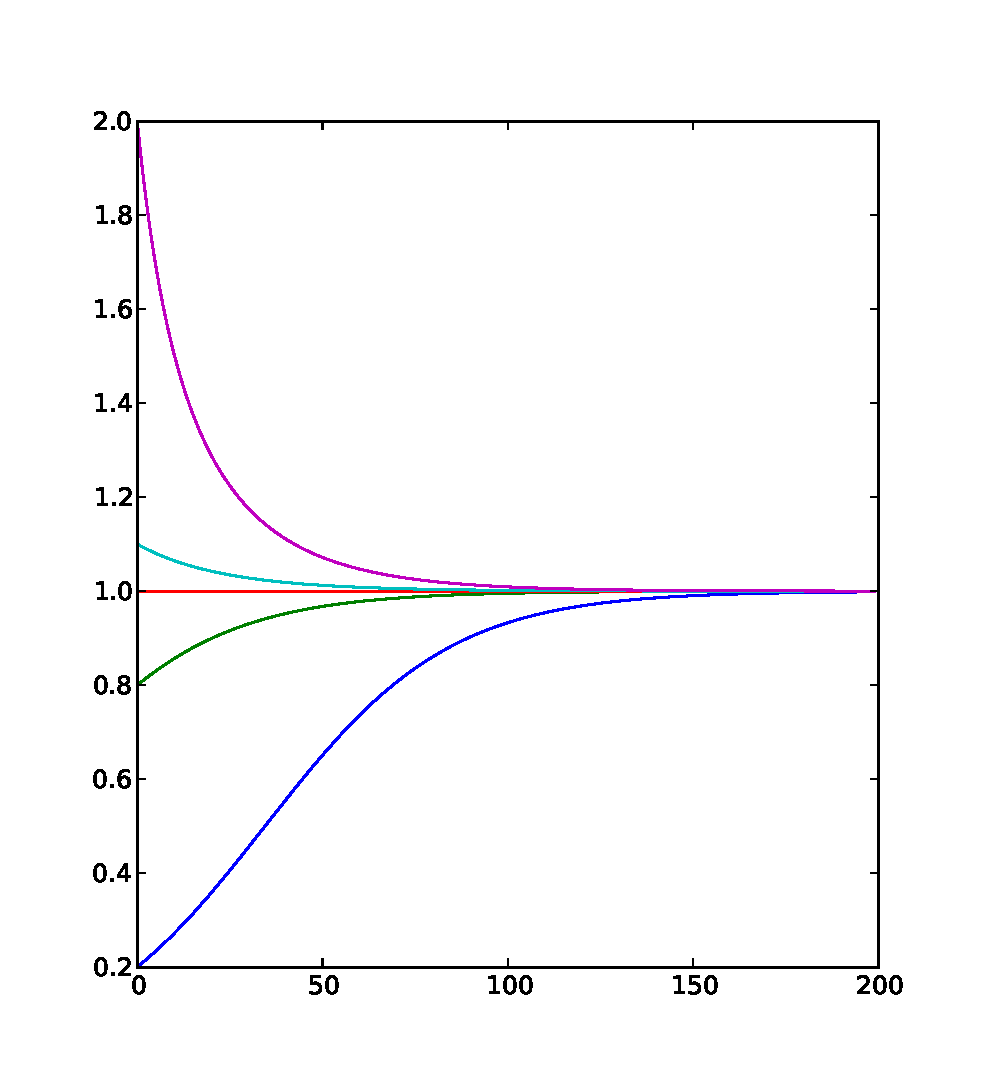
\includegraphics[scale=0.5]{logistic_diffeq_mu4_varyingx0.eps}
  \end{center}
  \caption{
    Plot of equation \pref{eq:logisticdiffeqsoln} with $\mu = 4$ and various $x_0$. 
  Note that regardless of the initial value, $x(t)$ converges to $1$.
}
  \label{fig:logistic_diffeq1}
\end{figure}

\begin{figure}[h]
  \begin{center}
    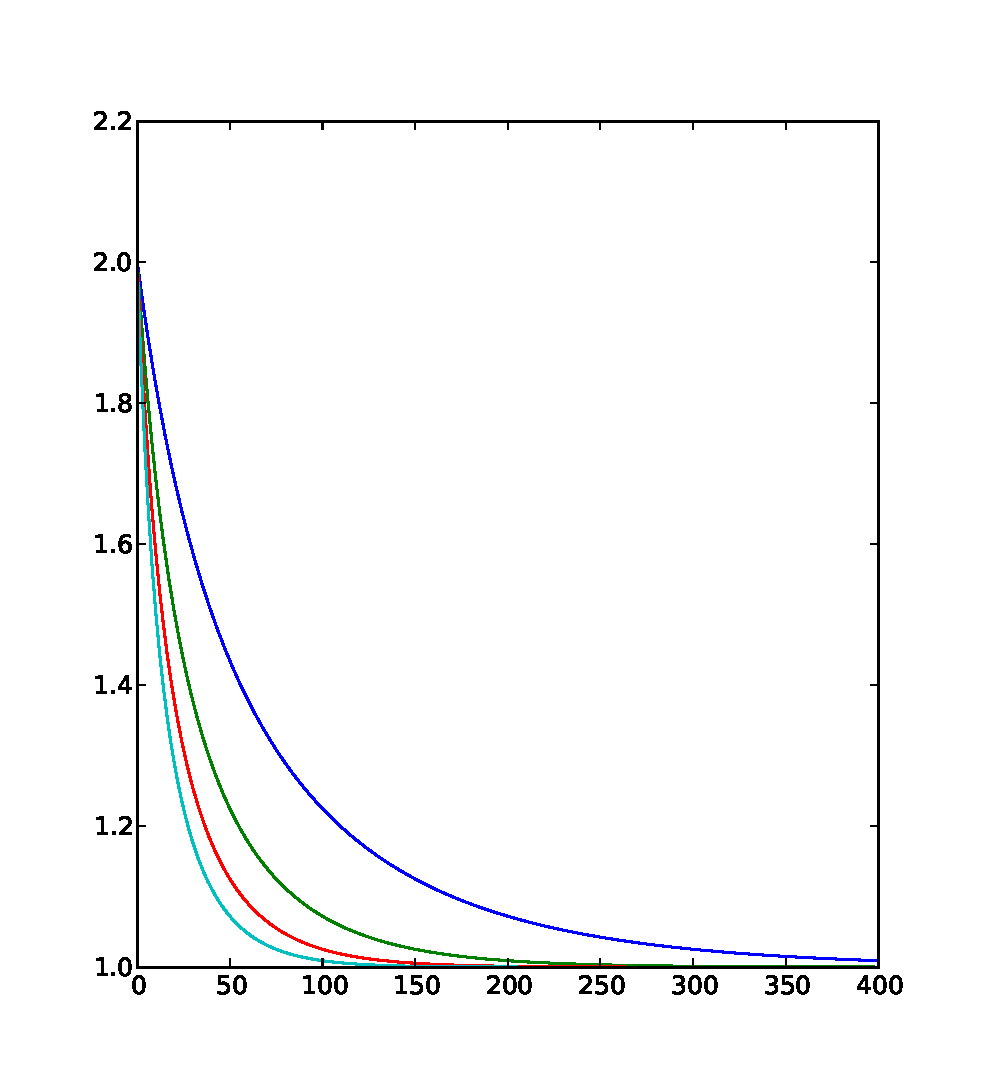
\includegraphics[scale=0.5]{logistic_diffeq_mu1234_x2.eps}
  \end{center}
  \caption{
    Plot of equation \pref{eq:logisticdiffeqsoln} with $x_0 = 2$ and various $\mu$ (1,2,3,4).
    As $\mu$ increases, $x(t)$ converges to $1$ faster.
    However, it does not alter the overall behaviour.
  }
  \label{fig:logistic_diffeq2}
\end{figure}

\begin{figure}[h]
  \begin{center}
    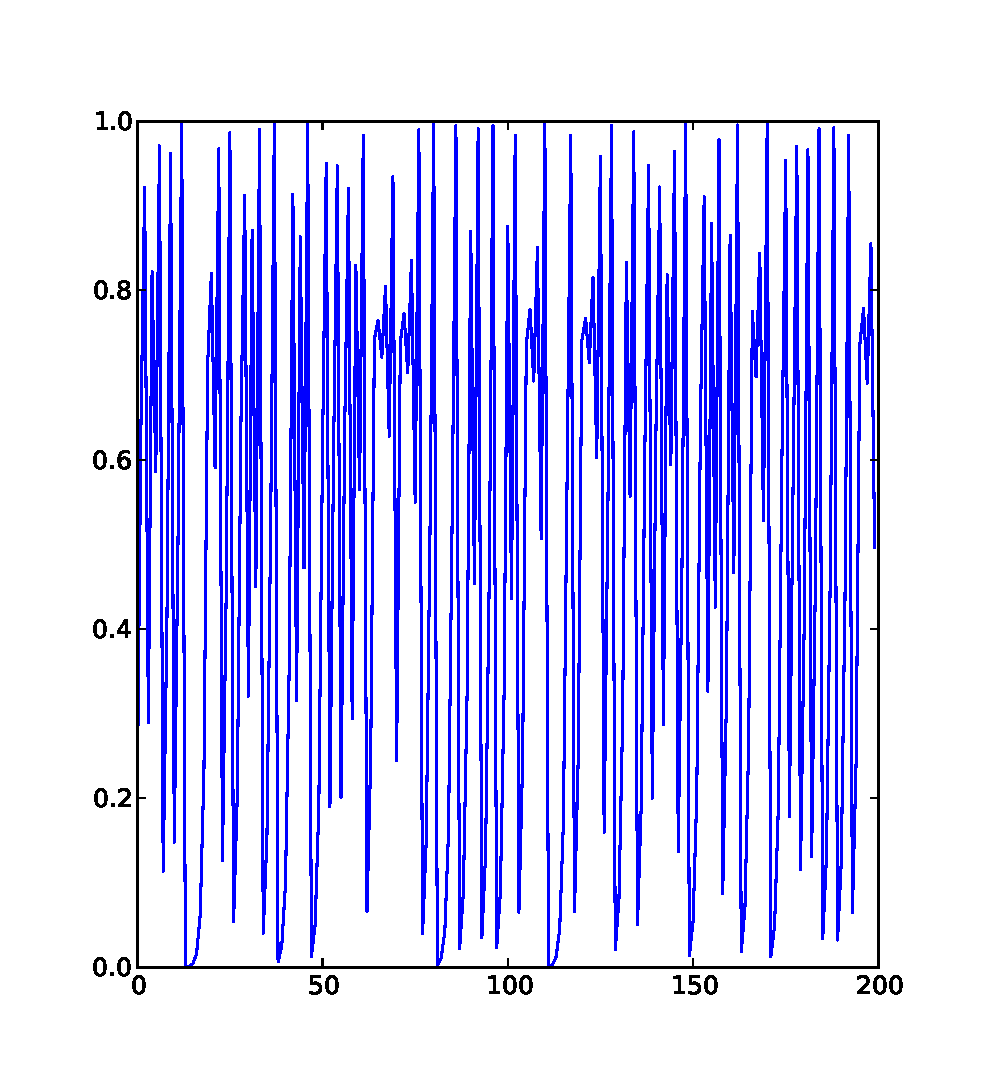
\includegraphics[scale=0.5]{logistic_map_mu4_x02.eps}
  \end{center}
  \caption{
    Chaotic map.
  }
  \label{fig:logistic_map_chaotic}
\end{figure}

We tend to label a dynamical systems as ``chaotic'' on an intuitive ground.
If the orbit looks (judged by our visual sense organ complex), the system is called chaotic.
In 1986, the Royal Society held an international conference on chaos and defined ``chaos'' as ``Stochastic behavior occurring in a deterministic system.'' \cite{stewart}
Two daunting Russian physicists famously said "A strange attractor seems strange only to a stranger."
(Boris Chirikov, Felix Izrailev)\cite{lorenzbook}

\bibliographystyle{plain}
\bibliography{../../bibliography/thesis}
\end{document}
